\documentclass[11pt]{article}
\usepackage[T1]{fontenc}
\usepackage[utf8]{inputenc}
\usepackage[a4paper,margin=1in]{geometry}
\usepackage{lmodern}
\usepackage{amsmath,amssymb,amsthm,mathtools}
\usepackage{booktabs,longtable,array,multirow}
\usepackage{enumitem}
\usepackage{graphicx}
\usepackage{xcolor}
\usepackage{float}
\usepackage{hyperref}
\usepackage{tikz}
\usepackage{pgfplots}
\usetikzlibrary{arrows.meta,positioning,shapes.geometric,calc,fit}
\pgfplotsset{compat=1.18}
\hypersetup{colorlinks=true,linkcolor=blue!50!black,urlcolor=blue!50!black}

\title{DEO Segmentation and Quantification Method\\Algorithm, Mathematical Definitions, and Metric Catalog}
\author{Lachlan Chen}
\date{2026-04-05}

\newcommand{\R}{\mathbb{R}}
\newcommand{\1}{\mathbf{1}}
\newcommand{\dx}{\,\mathrm{d}x}
\newcommand{\IoU}{\operatorname{IoU}}
\newcommand{\ovsmall}{\operatorname{ov}_{\mathrm{small}}}
\newcommand{\clip}{\operatorname{clip}}
\newcommand{\med}{\operatorname{median}}
\newcommand{\mean}{\operatorname{mean}}
\newcommand{\std}{\operatorname{std}}
\newcommand{\sem}{\operatorname{sem}}
\newcommand{\quantile}{\operatorname{Q}}
\newcommand{\dilate}{\operatorname{dilate}}
\newcommand{\erode}{\operatorname{erode}}
\newcommand{\openop}{\operatorname{open}}
\newcommand{\closeop}{\operatorname{close}}
\newcommand{\dist}{\operatorname{dist}}
\newcommand{\symdiff}{\triangle}
\newcommand{\normminmax}{\mathcal{N}}
\newcommand{\support}{M_{\mathrm{sup}}}
\newcommand{\unionmask}{U}
\newcommand{\edgefield}{E}
\newcommand{\signal}{S}
\newcommand{\gray}{I}
\newcommand{\labelmap}{L}

\begin{document}
\maketitle
\tableofcontents

\section{Scope}
This note documents the segmentation and quantification framework used across the DEO analysis outputs, especially the completed workflows for:
\begin{itemize}[leftmargin=1.5em]
  \item App80 Y-27632 concentration analysis,
  \item App65 alginate concentration analysis,
  \item App81 density analysis.
\end{itemize}

The aim is to explain, in one place:
\begin{itemize}[leftmargin=1.5em]
  \item the segmentation algorithm,
  \item the hybrid signal image and support mask,
  \item multiscale Cellpose plus large-mass recovery,
  \item candidate scoring and merge logic,
  \item every downstream metric in mathematical form.
\end{itemize}

This document defines the \emph{union} of the metrics currently used in the repository. Not every dataset uses every metric, but the formulas below cover the full implemented metric family.

\section{Notation}
Let the image domain be $\Omega \subset \mathbb{Z}^2$ and let the raw brightfield grayscale image be
\begin{equation}
\gray: \Omega \to [0,255].
\end{equation}
If the original TIFF is RGB, $\gray$ is obtained by RGB-to-grayscale conversion.

Let the final instance label image be
\begin{equation}
\labelmap: \Omega \to \{0,1,2,\dots,K\},
\end{equation}
where label $0$ denotes background and $K$ is the number of segmented organoid instances.

For instance $k \in \{1,\dots,K\}$, define the binary support set
\begin{equation}
\Omega_k = \{x \in \Omega : \labelmap(x)=k\}.
\end{equation}

Its basic geometry is:
\begin{align}
A_k &= |\Omega_k| && \text{area in pixels},\\
P_k &= \text{perimeter of } \Omega_k,\\
c_k &= \text{centroid of } \Omega_k.
\end{align}

The union of all segmented instances is
\begin{equation}
\unionmask = \bigcup_{k=1}^K \Omega_k.
\end{equation}

\section{Pipeline Overview}
\subsection{High-level flow}
\begin{figure}[H]
\centering
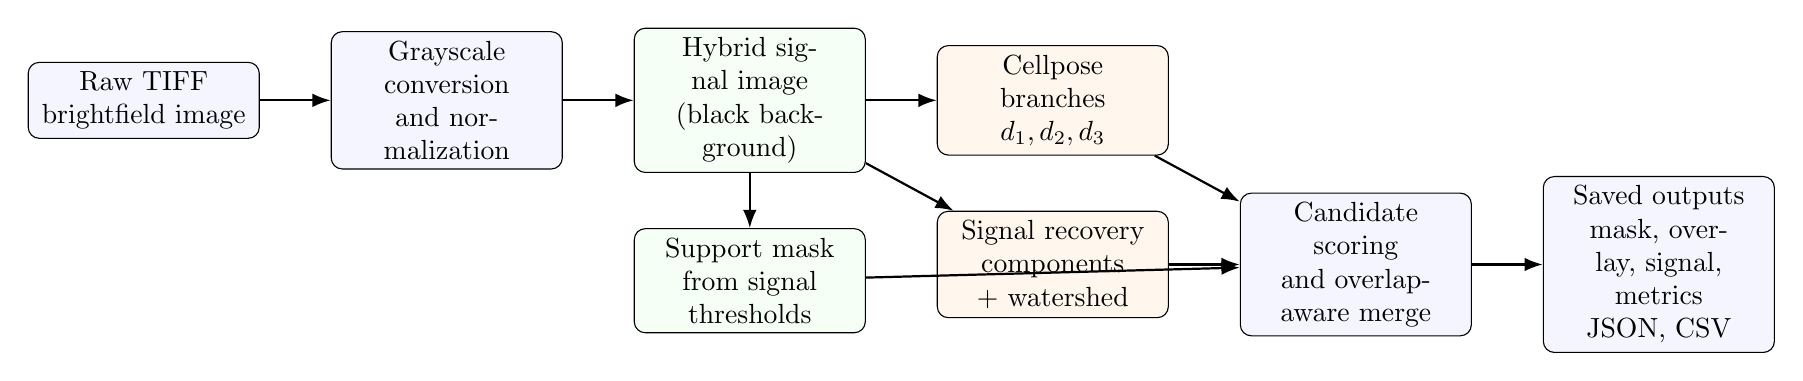
\begin{tikzpicture}[
  node distance=7mm and 9mm,
  box/.style={draw, rounded corners, align=center, minimum height=8mm, text width=27mm, fill=blue!4},
  box2/.style={draw, rounded corners, align=center, minimum height=8mm, text width=27mm, fill=green!4},
  box3/.style={draw, rounded corners, align=center, minimum height=8mm, text width=27mm, fill=orange!7},
  arrow/.style={-Latex, thick}
]
\node[box] (tif) {Raw TIFF\\brightfield image};
\node[box, right=of tif] (gray) {Grayscale conversion\\and normalization};
\node[box2, right=of gray] (signal) {Hybrid signal image\\(black background)};
\node[box2, below=of signal] (support) {Support mask\\from signal thresholds};
\node[box3, right=of signal] (cellpose) {Cellpose branches\\$d_1,d_2,d_3$};
\node[box3, below=of cellpose] (recover) {Signal recovery\\components + watershed};
\node[box, right=of recover] (merge) {Candidate scoring\\and overlap-aware merge};
\node[box, right=of merge] (out) {Saved outputs\\mask, overlay, signal,\\metrics JSON, CSV};

\draw[arrow] (tif) -- (gray);
\draw[arrow] (gray) -- (signal);
\draw[arrow] (signal) -- (cellpose);
\draw[arrow] (signal) -- (support);
\draw[arrow] (signal) -- (recover);
\draw[arrow] (support) -- (merge);
\draw[arrow] (cellpose) -- (merge);
\draw[arrow] (recover) -- (merge);
\draw[arrow] (merge) -- (out);
\end{tikzpicture}
\caption{High-level DEO segmentation workflow.}
\end{figure}

\subsection{Metric dependency chart}
\begin{figure}[H]
\centering
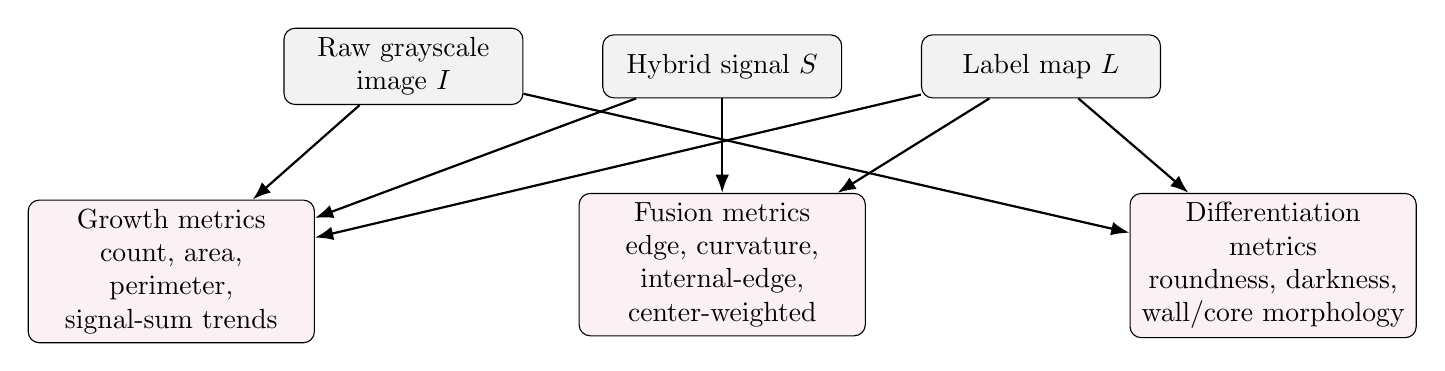
\begin{tikzpicture}[
  node distance=8mm and 10mm,
  src/.style={draw, rounded corners, align=center, minimum height=8mm, text width=28mm, fill=gray!10},
  grp/.style={draw, rounded corners, align=center, minimum height=8mm, text width=34mm, fill=purple!6},
  arrow/.style={-Latex, thick}
]
\node[src] (raw) {Raw grayscale image $\gray$};
\node[src, right=of raw] (sig) {Hybrid signal $\signal$};
\node[src, right=of sig] (lab) {Label map $\labelmap$};

\node[grp, below left=12mm and -4mm of raw] (growth) {Growth metrics\\count, area, perimeter,\\signal-sum trends};
\node[grp, below=12mm of sig] (fusion) {Fusion metrics\\edge, curvature,\\internal-edge, center-weighted};
\node[grp, below right=12mm and -4mm of lab] (diff) {Differentiation metrics\\roundness, darkness,\\wall/core morphology};

\draw[arrow] (raw) -- (growth);
\draw[arrow] (sig) -- (growth);
\draw[arrow] (sig) -- (fusion);
\draw[arrow] (lab) -- (growth);
\draw[arrow] (lab) -- (fusion);
\draw[arrow] (lab) -- (diff);
\draw[arrow] (raw) -- (diff);
\end{tikzpicture}
\caption{Which data products feed each metric family.}
\end{figure}

\section{Segmentation Algorithm}
\subsection{Hybrid signal image}
The saved black-background signal image is the main preprocessed representation used for support extraction and many downstream metrics.

Let $\tilde{I}$ denote CLAHE-enhanced grayscale:
\begin{equation}
\tilde{I} = \operatorname{CLAHE}(\gray).
\end{equation}

Let
\begin{align}
F &= G_{\sigma_f} * \tilde{I} && \text{foreground blur, small kernel},\\
B &= G_{\sigma_b} * \tilde{I} && \text{background blur, large kernel},\\
R &= B - F && \text{background-subtracted residual},\\
V &= 255 - F && \text{inverted foreground image}.
\end{align}

The min-max normalization to $[0,255]$ is denoted $\normminmax(\cdot)$. The final hybrid signal is
\begin{equation}
\signal = 0.45\,\normminmax(V) + 0.55\,\normminmax(R).
\end{equation}

In the current implementation, the typical fixed settings are:
\begin{itemize}[leftmargin=1.5em]
  \item CLAHE clip limit $=2.4$,
  \item foreground Gaussian blur kernel $=3\times3$,
  \item background Gaussian blur kernel $=31\times31$.
\end{itemize}

\subsection{Support mask}
A biologically informed support mask is extracted from the hybrid signal:
\begin{equation}
T_{\mathrm{sup}} = \max\left(T_{\mathrm{Otsu}}(\signal),\; \quantile_{0.58}(\signal)\right).
\end{equation}

The raw threshold mask is
\begin{equation}
M_{\mathrm{sup},0}(x)=\1[\signal(x)\ge T_{\mathrm{sup}}].
\end{equation}

Morphological cleanup then gives the final support mask $\support$:
\begin{equation}
\support = \closeop\bigl(\openop(M_{\mathrm{sup},0})\bigr).
\end{equation}

This is not the final segmentation. It is a support prior used to:
\begin{itemize}[leftmargin=1.5em]
  \item refine Cellpose masks,
  \item reject weak candidates,
  \item recover large irregular masses missed by Cellpose.
\end{itemize}

\subsection{Multiscale Cellpose branches}
Instead of one single diameter, the method evaluates several candidate scales per image:
\begin{equation}
\mathcal{D} = \{d_1,d_2,d_3\}.
\end{equation}

For each $d \in \mathcal{D}$, Cellpose produces a label image
\begin{equation}
\labelmap^{(d)} = \operatorname{Cellpose}(\gray; d).
\end{equation}

The actual triplets are dataset- and stage-specific. In App80, for example, later fused stages use substantially larger diameters than early cluster stages.

\subsection{Gradient image and candidate features}
A gradient magnitude image is computed from the CLAHE image or hybrid signal, depending on the code path. In either case, denote the normalized edge map by $\edgefield(x)\in[0,1]$.

For a candidate mask $\Omega_k$, the main candidate features are:
\paragraph{Support ratio}
\begin{equation}
r_{\mathrm{sup},k} = \frac{|\Omega_k \cap \dilate(\support)|}{|\Omega_k|}.
\end{equation}

\paragraph{Mean signal}
\begin{equation}
\mu_{\signal,k} = \frac{1}{|\Omega_k|}\sum_{x\in\Omega_k} \frac{\signal(x)}{255}.
\end{equation}

\paragraph{Boundary edge strength}
Let $\partial \Omega_k$ denote a morphological boundary of the candidate. Then
\begin{equation}
e_{\partial,k} = \frac{1}{|\partial \Omega_k|}\sum_{x\in\partial \Omega_k} \edgefield(x).
\end{equation}

\paragraph{Bounding-box fill ratio}
If the axis-aligned bounding box of $\Omega_k$ has width $w_k$ and height $h_k$, then
\begin{equation}
f_{\mathrm{box},k} = \frac{A_k}{w_k h_k}.
\end{equation}

\paragraph{Circularity}
\begin{equation}
\chi_k = \frac{4\pi A_k}{P_k^2}.
\end{equation}

\subsection{Candidate scoring}
A candidate score is formed as a weighted sum of biologically useful cues:
\begin{equation}
s_k = 1.85\,r_{\mathrm{sup},k} + 0.85\,\mu_{\signal,k} + 0.65\,e_{\partial,k} + 0.25\,f_{\mathrm{box},k} + b_{\mathrm{stage}} + b_{\mathrm{branch}}.
\end{equation}

Here:
\begin{itemize}[leftmargin=1.5em]
  \item $b_{\mathrm{stage}}$ is a stage-dependent bonus,
  \item $b_{\mathrm{branch}}$ is a small branch-preference term.
\end{itemize}

These bonuses are empirical. They are used to encourage candidates that better match the known morphology of a stage, for example early clusters versus large fused irregular masses.

\subsection{Signal-based large-mass recovery}
Cellpose alone often misses very large irregular fused structures. To recover them, the method also thresholds the hybrid signal directly.

For a quantile $q$, define the binary thresholded signal mask
\begin{equation}
B_q(x) = \1[\signal(x) \ge \quantile_q(\signal)].
\end{equation}

Then apply morphological close/open, border clearing, and hole filling to obtain connected components.

A second recovery path uses watershed seeds derived from the distance transform:
\begin{equation}
D_q(x) = \dist(B_q)(x),
\end{equation}
and seed points are selected by
\begin{equation}
Z_q(x) = \1\left[D_q(x) > \tau \max_{y\in\Omega} D_q(y)\right].
\end{equation}

Watershed is then run on the thresholded region, producing additional large-object candidates.

\subsection{Candidate merge logic}
The final mask set is built by overlap-aware merging across all branches.

For two masks $A$ and $B$:
\begin{align}
\IoU(A,B) &= \frac{|A\cap B|}{|A\cup B|},\\
\ovsmall(A,B) &= \frac{|A\cap B|}{\min(|A|,|B|)}.
\end{align}

The implemented logic is approximately:
\begin{itemize}[leftmargin=1.5em]
  \item if $\ovsmall>0.80$ or $\IoU>0.60$, treat the masks as competing explanations of the same object,
  \item replace the previous mask if the new one has clearly better score or clearly better supported larger area,
  \item reject small redundant fragments when they overlap a much larger accepted mask.
\end{itemize}

\subsection{Saved outputs}
Per image, the pipeline saves:
\begin{itemize}[leftmargin=1.5em]
  \item \texttt{*\_mask\_16bit.png}: integer instance labels,
  \item \texttt{*\_instance\_rgb.png}: random-color instance rendering,
  \item \texttt{*\_overlay.png}: source image with instance overlay,
  \item \texttt{*\_signal.png}: hybrid signal image,
  \item \texttt{*\_metrics.json}: per-image quantitative summary,
  \item \texttt{*\_segmentation\_stats.json}: segmentation provenance and branch details.
\end{itemize}

\section{Geometric and Spatial Primitives}
\subsection{Distance transform and centrality}
For instance $\Omega_k$, let the Euclidean distance transform inside the instance be
\begin{equation}
D_k(x) = \dist(\Omega_k)(x), \qquad x\in\Omega_k.
\end{equation}

The normalized centrality field is
\begin{equation}
C_k(x) = \frac{D_k(x)}{\max_{y\in\Omega_k} D_k(y)} \in [0,1].
\end{equation}

Thus:
\begin{itemize}[leftmargin=1.5em]
  \item $C_k(x)\approx 0$ near the object boundary,
  \item $C_k(x)=1$ at the deepest interior point(s).
\end{itemize}

\subsection{Exponential center weighting}
To emphasize interior edge structure, a centrality weight is defined as
\begin{equation}
w_{\alpha}(c)=\frac{e^{\alpha c}-1}{e^{\alpha}-1}, \qquad c\in[0,1].
\end{equation}

The current implementation uses $\alpha=5$.

\begin{figure}[H]
\centering
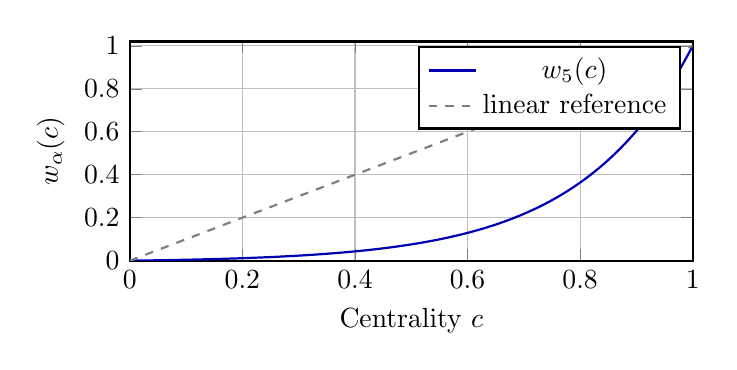
\begin{tikzpicture}
\begin{axis}[
  width=0.72\textwidth,
  height=0.36\textwidth,
  xlabel={Centrality $c$},
  ylabel={$w_{\alpha}(c)$},
  xmin=0, xmax=1,
  ymin=0, ymax=1.02,
  domain=0:1,
  samples=200,
  grid=both,
  thick
]
\addplot[blue!70!black] {(exp(5*x)-1)/(exp(5)-1)};
\addplot[dashed,gray] {x};
\legend{$w_{5}(c)$, linear reference}
\end{axis}
\end{tikzpicture}
\caption{Exponential center weighting used in the center-weighted internal-edge metrics.}
\end{figure}

\subsection{Wall/core decomposition}
For differentiation-darkness metrics, each organoid is split into a wall band and a core.

If $A_k$ is the object area, its equivalent radius is
\begin{equation}
r_k^{\mathrm{eq}} = \sqrt{\frac{A_k}{\pi}}.
\end{equation}

The erosion band thickness is
\begin{equation}
t_k = \clip\left(\operatorname{round}(0.12\,r_k^{\mathrm{eq}}), 5, 30\right).
\end{equation}

Then:
\begin{align}
\Omega_k^{\mathrm{core}} &= \erode(\Omega_k; t_k),\\
\Omega_k^{\mathrm{wall}} &= \Omega_k \setminus \Omega_k^{\mathrm{core}}.
\end{align}

\begin{figure}[H]
\centering
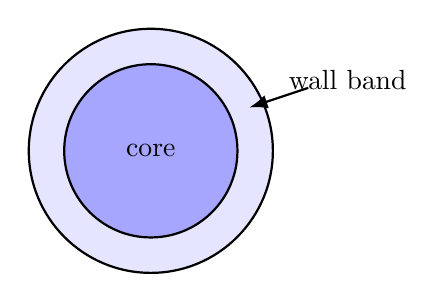
\begin{tikzpicture}[scale=1.0]
\fill[blue!10] (0,0) circle (1.55);
\fill[blue!35] (0,0) circle (1.10);
\draw[thick] (0,0) circle (1.55);
\draw[thick] (0,0) circle (1.10);
\node at (0,0) {core};
\node at (2.5,0.9) {wall band};
\draw[-Latex,thick] (2.0,0.8) -- (1.25,0.55);
\end{tikzpicture}
\caption{Adaptive wall/core decomposition for darkness metrics.}
\end{figure}

\section{Metric Definitions}
This section defines the union of the metrics currently implemented across the DEO analysis workflows.

\subsection{Growth metrics}
\paragraph{Count}
\begin{equation}
N = K.
\end{equation}
This is the number of segmented instances in one image.

\paragraph{Total segmented area}
\begin{equation}
A_{\mathrm{tot}} = \sum_{k=1}^{K} A_k.
\end{equation}
This is the main segmentation-based growth proxy.

\paragraph{Average perimeter}
\begin{equation}
\bar{P} = \frac{1}{K}\sum_{k=1}^{K} P_k,
\end{equation}
with the convention $\bar{P}=0$ if $K=0$.

\paragraph{Signal sum intensity}
The hybrid-signal intensity sum is computed over the full image:
\begin{equation}
I_{\mathrm{sum}} = \sum_{x\in\Omega} \signal(x).
\end{equation}
It is an exploratory morphology-sensitive intensity proxy.

\paragraph{Reciprocal signal sum}
\begin{equation}
I_{\mathrm{sum}}^{-1} = \frac{1}{I_{\mathrm{sum}}}.
\end{equation}
This is used when an inverse scale is visually easier to interpret.

\paragraph{Relative change of signal sum}
For timepoint $t$:
\begin{equation}
\Delta_{\mathrm{sum}}^{\mathrm{rel}}(t) = \frac{I_{\mathrm{sum}}(t)-I_{\mathrm{sum}}(t-1)}{I_{\mathrm{sum}}(t-1)}.
\end{equation}

\paragraph{Relative change of reciprocal signal sum}
\begin{equation}
\Delta_{\mathrm{recip}}^{\mathrm{rel}}(t) = \frac{I_{\mathrm{sum}}^{-1}(t)-I_{\mathrm{sum}}^{-1}(t-1)}{I_{\mathrm{sum}}^{-1}(t-1)}.
\end{equation}

\subsection{Fusion metrics: boundary and shape core}
\paragraph{Boundary edge intensity}
Let $B_{\partial}$ be the union of morphological boundaries of all instances. Then
\begin{equation}
E_{\partial} = \frac{1}{|B_{\partial}|}\sum_{x\in B_{\partial}} \edgefield(x).
\end{equation}
This is saved as \texttt{edge\_intensity}.

\paragraph{Per-instance circularity}
For each instance:
\begin{equation}
\chi_k = \frac{4\pi A_k}{P_k^2}.
\end{equation}
This is the standard area-perimeter circularity.

\paragraph{Image-level curvature}
The project-level curvature proxy is the area-weighted mean circularity:
\begin{equation}
C = \frac{1}{A_{\mathrm{tot}}}\sum_{k=1}^{K} A_k\chi_k.
\end{equation}
This is saved as \texttt{curvature}.

\paragraph{Min-max-with-floor normalization}
For any per-image scalar $v_i$, define
\begin{equation}
\operatorname{norm}_{\eta}(v_i) = \max\left(\eta, \frac{v_i-v_{\min}}{v_{\max}-v_{\min}}\right),
\end{equation}
where $\eta=0.1$ in the current workflow, and $v_{\min},v_{\max}$ are taken over the batch being summarized.

This produces:
\begin{align}
N_{\mathrm{norm}} &= \operatorname{norm}_{0.1}(N),\\
C_{\mathrm{norm}} &= \operatorname{norm}_{0.1}(C),\\
E_{\mathrm{norm}} &= \operatorname{norm}_{0.1}(E_{\partial}).
\end{align}

\paragraph{Normalized edge over count and curvature}
\begin{equation}
M_{\mathrm{norm}} = \frac{E_{\mathrm{norm}}}{N_{\mathrm{norm}}\,C_{\mathrm{norm}}}.
\end{equation}
This is \texttt{normalized\_edge\_over\_count\_curvature}.

\paragraph{Inverse edge-count-curvature product}
\begin{equation}
M_{\mathrm{inv}} = \frac{1}{E_{\partial}\,N\,C}.
\end{equation}
This is \texttt{inverse\_edge\_count\_curvature}.

\paragraph{Edge density}
Let $T$ be a tissue mask built from a residual brightfield heuristic, and let $B_E$ be the Canny edge set inside the blurred grayscale image. Then
\begin{equation}
\rho_E = \frac{|B_E \cap T|}{|T|}.
\end{equation}
This is \texttt{edge\_density}.

\paragraph{Reciprocal edge density}
\begin{equation}
\rho_E^{-1} = \frac{1}{\max(\rho_E,\varepsilon)},
\end{equation}
where $\varepsilon$ is a small numerical stabilizer.

\paragraph{Gradient mean}
If $G_x,G_y$ are Sobel derivatives and $G=\sqrt{G_x^2+G_y^2}$, then
\begin{equation}
\bar{G}_T = \frac{1}{|T|}\sum_{x\in T} G(x).
\end{equation}
This is \texttt{gradient\_mean}.

\paragraph{Reciprocal gradient mean}
\begin{equation}
\bar{G}_T^{-1} = \frac{1}{\max(\bar{G}_T,\varepsilon)}.
\end{equation}

\subsection{Fusion metrics: internal-edge and spatial redistribution}
These metrics test the biological idea that stronger fusion corresponds to edge structure moving from the outer boundary into the interior of segmented organoids.

\paragraph{Central inside edge mean}
Using centrality $C_k(x)$,
\begin{equation}
E_{\mathrm{cen}} = \frac{\sum_{k=1}^{K}\sum_{x\in\Omega_k} \edgefield(x)\,C_k(x)}{\sum_{k=1}^{K}\sum_{x\in\Omega_k} C_k(x)}.
\end{equation}
This is \texttt{central\_inside\_edge\_mean}.

\paragraph{Peripheral inside edge mean}
\begin{equation}
E_{\mathrm{per}} = \frac{\sum_{k=1}^{K}\sum_{x\in\Omega_k} \edgefield(x)\,(1-C_k(x))}{\sum_{k=1}^{K}\sum_{x\in\Omega_k} (1-C_k(x))}.
\end{equation}
This is \texttt{peripheral\_inside\_edge\_mean}.

\paragraph{Outer-ring edge mean}
Let
\begin{equation}
R_{\mathrm{out}} = \dilate(\unionmask) \setminus \unionmask.
\end{equation}
Then
\begin{equation}
E_{\mathrm{out}} = \frac{1}{|R_{\mathrm{out}}|}\sum_{x\in R_{\mathrm{out}}} \edgefield(x).
\end{equation}
This is \texttt{outer\_ring\_edge\_mean}.

\paragraph{Central inside fraction}
\begin{equation}
F_{\mathrm{cen}} = \frac{E_{\mathrm{cen}}}{E_{\mathrm{cen}}+E_{\mathrm{per}}}.
\end{equation}
This is \texttt{central\_inside\_fraction}.

\paragraph{Central-to-peripheral ratio}
\begin{equation}
R_{\mathrm{cen/per}} = \frac{E_{\mathrm{cen}}}{E_{\mathrm{per}}}.
\end{equation}
This is \texttt{central\_inside\_over\_peripheral}.

\paragraph{Central-to-outer ratio}
\begin{equation}
R_{\mathrm{cen/out}} = \frac{E_{\mathrm{cen}}}{E_{\mathrm{out}}}.
\end{equation}
This is \texttt{central\_inside\_over\_outer}.

\paragraph{Peripheral-to-central ratio}
\begin{equation}
R_{\mathrm{per/cen}} = \frac{E_{\mathrm{per}}}{E_{\mathrm{cen}}}.
\end{equation}
This is \texttt{peripheral\_over\_central}.

\paragraph{Center-weighted edge sum}
Using the exponential weight $w_\alpha$,
\begin{equation}
S_{\mathrm{cw}} = \sum_{k=1}^{K}\sum_{x\in\Omega_k} \edgefield(x)\,w_{\alpha}(C_k(x)).
\end{equation}
This is \texttt{center\_weighted\_edge\_sum}.

\paragraph{Center-weighted edge weight sum}
\begin{equation}
W_{\mathrm{cw}} = \sum_{k=1}^{K}\sum_{x\in\Omega_k} w_{\alpha}(C_k(x)).
\end{equation}
This is \texttt{center\_weighted\_edge\_weight\_sum}.

\paragraph{Center-weighted edge mean}
\begin{equation}
\bar{E}_{\mathrm{cw}} = \frac{S_{\mathrm{cw}}}{W_{\mathrm{cw}}}.
\end{equation}
This is \texttt{center\_weighted\_edge\_mean}.

\paragraph{Mean instance center-weighted edge sum}
If
\begin{equation}
S_{\mathrm{cw},k}=\sum_{x\in\Omega_k} \edgefield(x)\,w_{\alpha}(C_k(x)),
\end{equation}
then
\begin{equation}
\bar{S}_{\mathrm{cw,inst}} = \frac{1}{K}\sum_{k=1}^{K} S_{\mathrm{cw},k}.
\end{equation}
This is \texttt{instance\_center\_weighted\_edge\_sum\_mean}.

\paragraph{Area-normalized center-weighted edge}
Define, for each instance,
\begin{equation}
a_k = \frac{S_{\mathrm{cw},k}}{A_k}.
\end{equation}
Then the saved summary statistics are:
\begin{align}
\bar{a} &= \frac{1}{K}\sum_{k=1}^{K} a_k && \texttt{area\_normalized\_center\_weighted\_edge\_instance\_mean},\\
\std(a_k) &&& \texttt{area\_normalized\_center\_weighted\_edge\_instance\_std},\\
\operatorname{median}(a_k) &&& \texttt{area\_normalized\_center\_weighted\_edge\_instance\_median}.
\end{align}

\subsection{Differentiation metrics: geometric roundness}
These metrics aim to capture how much each segmented object deviates from a circle of equal area centered at the object centroid.

\paragraph{Reference circle}
For object $\Omega_k$ with centroid $c_k$ and area $A_k$, define the same-area radius
\begin{equation}
r_k = \sqrt{\frac{A_k}{\pi}}.
\end{equation}
The reference circle is
\begin{equation}
\Gamma_k = \{x\in\Omega : \|x-c_k\|_2 \le r_k\}.
\end{equation}

\paragraph{Absolute area deviation from the reference circle}
\begin{equation}
D_k = |\Omega_k \symdiff \Gamma_k|.
\end{equation}
This is the symmetric-difference area in pixels.

\paragraph{Normalized deviation}
\begin{equation}
\delta_k = \frac{D_k}{|\Omega_k \cup \Gamma_k|}.
\end{equation}
This is \texttt{roundness\_deviation\_norm} at the per-object level.

\paragraph{Roundness}
\begin{equation}
R_k = \max(0, 1-\delta_k).
\end{equation}
This is the object-level roundness score.

\paragraph{Image-level roundness}
\begin{equation}
R = \frac{1}{A_{\mathrm{tot}}}\sum_{k=1}^{K} A_k R_k.
\end{equation}
This is \texttt{roundness}.

\paragraph{Image-level normalized deviation}
\begin{equation}
\delta = \frac{1}{A_{\mathrm{tot}}}\sum_{k=1}^{K} A_k\delta_k.
\end{equation}
This is \texttt{roundness\_deviation\_norm} at image level.

\paragraph{Total deviation pixels}
\begin{equation}
D_{\mathrm{tot}} = \sum_{k=1}^{K} D_k.
\end{equation}
This is \texttt{roundness\_deviation\_px\_total}.

\subsection{Differentiation metrics: darkness and wall thickening}
These metrics target darker, thickened epithelial walls and darker budded structures associated with stronger differentiation.

\paragraph{Background grayscale median}
Let the background region be the complement of a dilated union mask:
\begin{equation}
B = \Omega \setminus \dilate(\unionmask).
\end{equation}
The background median is
\begin{equation}
b = \med\{\gray(x): x\in B\}.
\end{equation}
This is \texttt{background\_gray\_median}.

\paragraph{Normalized darkness field}
Darkness is defined relative to the background median:
\begin{equation}
D(x) = \clip\left(\frac{b-\gray(x)}{\max(b,1)}, 0, 1\right).
\end{equation}
A darker pixel relative to background has a larger $D(x)$.

\paragraph{Organoid darkness mean}
\begin{equation}
\bar{D}_{\unionmask} = \frac{1}{|\unionmask|}\sum_{x\in\unionmask} D(x).
\end{equation}
This is \texttt{organoid\_darkness\_mean}.

\paragraph{Organoid darkness upper quantiles}
\begin{align}
D_{0.90} &= \quantile_{0.90}\{D(x):x\in\unionmask\},\\
D_{0.95} &= \quantile_{0.95}\{D(x):x\in\unionmask\}.
\end{align}
These are \texttt{organoid\_darkness\_p90} and \texttt{organoid\_darkness\_p95}.

\paragraph{Very dark area ratio}
With threshold $\tau_D=0.35$,
\begin{equation}
R_{\mathrm{dark}>0.35} = \frac{|\{x\in\unionmask : D(x) > 0.35\}|}{|\unionmask|}.
\end{equation}
This is \texttt{very\_dark\_area\_ratio\_gt035}.

\paragraph{Wall darkness mean}
Let
\begin{equation}
\unionmask^{\mathrm{wall}} = \bigcup_{k=1}^{K} \Omega_k^{\mathrm{wall}}.
\end{equation}
Then
\begin{equation}
\bar{D}_{\mathrm{wall}} = \frac{1}{|\unionmask^{\mathrm{wall}}|}\sum_{x\in\unionmask^{\mathrm{wall}}} D(x).
\end{equation}
This is \texttt{wall\_darkness\_mean}.

\paragraph{Wall darkness 90th percentile}
\begin{equation}
D_{\mathrm{wall},0.90} = \quantile_{0.90}\{D(x): x\in\unionmask^{\mathrm{wall}}\}.
\end{equation}
This is \texttt{wall\_darkness\_p90}.

\paragraph{Core darkness mean}
Let
\begin{equation}
\unionmask^{\mathrm{core}} = \bigcup_{k=1}^{K} \Omega_k^{\mathrm{core}}.
\end{equation}
Then
\begin{equation}
\bar{D}_{\mathrm{core}} = \frac{1}{|\unionmask^{\mathrm{core}}|}\sum_{x\in\unionmask^{\mathrm{core}}} D(x).
\end{equation}
This is \texttt{core\_darkness\_mean}.

\paragraph{Wall/core darkness ratio}
\begin{equation}
R_{\mathrm{wall/core}} = \frac{\bar{D}_{\mathrm{wall}}}{\max(\bar{D}_{\mathrm{core}}, 10^{-6})}.
\end{equation}
This is \texttt{wall\_core\_darkness\_ratio}.

\paragraph{Pixel-count bookkeeping}
The following are stored for completeness:
\begin{align}
N_{\mathrm{pix,organoid}} &= |\unionmask|,\\
N_{\mathrm{pix,wall}} &= |\unionmask^{\mathrm{wall}}|,\\
N_{\mathrm{pix,core}} &= |\unionmask^{\mathrm{core}}|.
\end{align}
These correspond to \texttt{organoid\_pixel\_count}, \texttt{wall\_pixel\_count}, and \texttt{core\_pixel\_count}.

\section{Interpretation by Biological Question}
\subsection{Growth}
The strongest growth-facing metrics are usually:
\begin{itemize}[leftmargin=1.5em]
  \item $A_{\mathrm{tot}}$ (total segmented area),
  \item $N$ (count, with caution),
  \item $I_{\mathrm{sum}}$ and its temporal changes.
\end{itemize}

\subsection{Fusion}
The strongest fusion-facing metrics are usually:
\begin{itemize}[leftmargin=1.5em]
  \item $M_{\mathrm{norm}} = E_{\mathrm{norm}}/(N_{\mathrm{norm}}C_{\mathrm{norm}})$,
  \item $M_{\mathrm{inv}} = 1/(E_{\partial}NC)$,
  \item $E_{\mathrm{cen}}/E_{\mathrm{per}}$,
  \item center-weighted internal-edge metrics.
\end{itemize}

These are based on the idea that stronger fusion moves edge structure from the outer organoid boundary toward the organoid interior.

\subsection{Differentiation}
The strongest differentiation-facing metrics are usually:
\begin{itemize}[leftmargin=1.5em]
  \item roundness and roundness-deviation metrics,
  \item organoid darkness upper quantiles,
  \item very-dark area ratio,
  \item wall darkness and wall/core darkness ratio.
\end{itemize}

These are aligned with thicker epithelial walls, darker appearance, and budded or irregular differentiated morphologies.

\section{Implementation Constants Used in Current Code}
\begin{table}[H]
\centering
\small
\begin{tabular}{@{}lll@{}}
\toprule
Quantity & Typical value & Role \\
\midrule
Hybrid signal foreground blur & $3\times3$ Gaussian & local support \\
Hybrid signal background blur & $31\times31$ Gaussian & background estimate \\
Hybrid signal mixing weights & $0.45, 0.55$ & inverted + residual blend \\
Support threshold quantile & $0.58$ & signal support floor \\
Normalization floor & $0.1$ & stable composite metrics \\
Very dark threshold & $0.35$ & dark-area ratio \\
Wall band scale & $0.12\,r_k^{\mathrm{eq}}$ & wall/core split \\
Wall band clamp & $5$ to $30$ px & wall/core robustness \\
Center-weight exponent & $\alpha=5$ & stronger interior emphasis \\
\bottomrule
\end{tabular}
\caption{Important fixed constants used in the current metric implementations.}
\end{table}

\section{Repository Mapping}
The method described here corresponds primarily to these code families:
\begin{itemize}[leftmargin=1.5em]
  \item \texttt{analysis-tools/app80\_first\_replicate\_multiscale\_cellpose/}
  \item \texttt{analysis-tools/app65\_alginate\_multiscale\_cellpose/}
  \item \texttt{analysis-tools/app81\_density\_multiscale\_cellpose/}
\end{itemize}

The metric union defined here matches the project-level metric catalog documented separately in:
\begin{itemize}[leftmargin=1.5em]
  \item \texttt{references/deo\_metric\_catalog\_growth\_fusion\_differentiation.md}
\end{itemize}

\section{Practical Summary}
The DEO workflow is best understood as a two-layer system:
\begin{enumerate}[leftmargin=1.8em]
  \item a segmentation layer that combines multiscale Cellpose with deterministic signal-based large-mass recovery,
  \item a quantification layer that maps the saved mask and signal outputs into growth, fusion, and differentiation metrics.
\end{enumerate}

The segmentation architecture is reusable, but the diameter schedules and stage-specific thresholds are dataset-specific. The metric layer is more portable, because it operates on the saved label map, hybrid signal image, and original grayscale image.

\end{document}
